\documentclass[10pt,a4paper]{article}

\usepackage[T1]{fontenc}
\usepackage{tgheros}
\renewcommand{\familydefault}{\sfdefault}

\usepackage[
  top=18mm,
  bottom=18mm,
  left=12mm,
  right=12mm,
  headheight=12pt,
  headsep=3mm,
  footskip=8mm
]{geometry}
\usepackage{graphicx}
\usepackage{booktabs}
\usepackage{tabularx}
\usepackage{array}
\usepackage[table]{xcolor}
\usepackage{tikz}
\usetikzlibrary{arrows.meta,positioning,fit}
\usepackage[numbers,sort&compress]{natbib}
\usepackage{hyperref}
\usepackage{microtype}
\usepackage{enumitem}
\usepackage{caption}
\usepackage{fancyhdr}
\usepackage{ragged2e}

\definecolor{blue}{HTML}{2563EB}
\definecolor{bluepale}{HTML}{EFF6FF}
\definecolor{green}{HTML}{15803D}
\definecolor{greenpale}{HTML}{F0FDF4}
\definecolor{orange}{HTML}{D97706}
\definecolor{orangepale}{HTML}{FFF7ED}
\definecolor{ink}{HTML}{0F172A}
\definecolor{muted}{HTML}{475569}
\definecolor{line}{HTML}{CBD5E1}
\definecolor{surface}{HTML}{F8FAFC}

\hypersetup{
  colorlinks=true,
  linkcolor=blue,
  citecolor=blue,
  urlcolor=blue,
  pdftitle={Loreley: Evolution Dynamics Technical Report},
  pdfauthor={Mohan Chen}
}

\pagestyle{fancy}
\fancyhf{}
\fancyhead[L]{\color{muted}\footnotesize LORELEY TECHNICAL REPORT}
\fancyhead[R]{\color{muted}\footnotesize Evolution dynamics}
\fancyfoot[C]{\color{muted}\footnotesize \thepage\ / 4}
\renewcommand{\headrulewidth}{0.35pt}
\renewcommand{\footrulewidth}{0pt}
\setlength{\parindent}{0pt}
\setlength{\parskip}{3.2pt}
\setlength{\emergencystretch}{2em}
\setlist[itemize]{leftmargin=1.2em,itemsep=1pt,topsep=2pt,parsep=0pt}
\captionsetup{font=small,labelfont=bf,skip=3pt}
\newcolumntype{Y}{>{\RaggedRight\arraybackslash}X}
\newcolumntype{C}[1]{>{\centering\arraybackslash}p{#1}}

\newcommand{\pagetitle}[2]{%
  {\color{blue}\fontsize{11}{12}\selectfont\bfseries #1}\par
  {\color{ink}\fontsize{20}{22}\selectfont\bfseries #2}\vspace{3pt}\par
  {\color{line}\rule{\textwidth}{0.65pt}}\vspace{4pt}
}

\newcommand{\metriccard}[3]{%
  \begin{minipage}[t][19mm][c]{0.235\textwidth}
    \centering
    {\color{#3}\fontsize{20}{21}\selectfont\bfseries #1}\par
    {\color{muted}\scriptsize #2}
  \end{minipage}%
}

\newcommand{\callout}[2]{%
  \colorbox{bluepale}{%
    \parbox{\dimexpr\linewidth-2\fboxsep\relax}{%
      \vspace{2pt}{\color{blue}\bfseries #1}\quad #2\vspace{2pt}%
    }%
  }%
}

\newcommand{\decisionbox}[3]{%
  \begin{minipage}[t]{0.315\textwidth}
    \vspace{0pt}%
    \colorbox{#1}{\parbox{\dimexpr\linewidth-2\fboxsep\relax}{%
      \RaggedRight\vspace{3pt}{\bfseries #2}\par\small #3\vspace{3pt}}}
  \end{minipage}%
}

\begin{document}

% -----------------------------------------------------------------------------
% Page 1
% -----------------------------------------------------------------------------
\thispagestyle{fancy}
\vspace*{-3mm}
{\color{ink}\fontsize{25}{27}\selectfont\bfseries
Loreley: Parallel, Multi-Branch Evolution\par
of Complete Code Repositories}\par
\vspace{2pt}
{\color{muted}\fontsize{12}{14}\selectfont
Quality over wall-clock time and longer searches}\hfill
{\small Mohan Chen \textperiodcentered\ 2026-09}\par
\vspace{5pt}

\colorbox{surface}{\parbox{\dimexpr\textwidth-2\fboxsep\relax}{%
\vspace{3pt}
\metriccard{2.78$\times$}{Champion / QD time for 48 jobs\par Paired geometric mean}{blue}\hfill
\metriccard{7/7}{Blocks where QD leads\par when its 48 jobs finish}{green}\hfill
\metriccard{6/7}{QD blocks reaching\par the +0.50\% threshold}{blue}\hfill
\metriccard{3--42}{Jobs between a retained branch\par and its final descendant}{orange}
\vspace{3pt}}}

\vspace{6pt}
\callout{Main result}{Loreley's quality-diversity (QD) search advances several branches in parallel and retains evaluated intermediate states as future parents. It reaches useful improvements sooner than Sequential Champion. At the same budget of 48 jobs, Sequential Champion has a slightly higher mean endpoint.}

\vspace{6pt}
{\color{ink}\large\bfseries How the three strategies grow their lineages}\par
\vspace{3pt}
\begin{center}
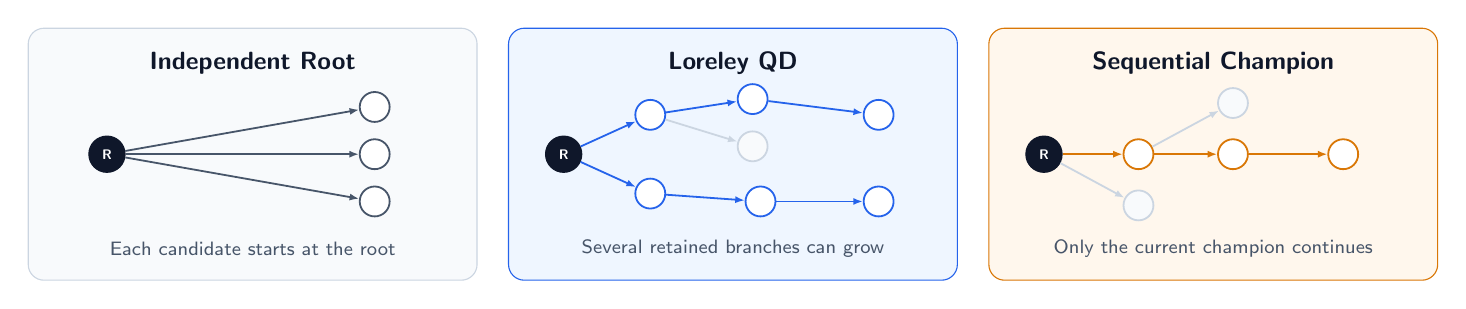
\begin{tikzpicture}[
  x=1mm,
  y=1mm,
  root/.style={
    circle,minimum size=4.6mm,inner sep=0pt,draw=ink,fill=ink,
    text=white,font=\tiny\bfseries
  },
  state/.style={
    circle,minimum size=3.8mm,inner sep=0pt,line width=0.65pt
  },
  independent/.style={state,draw=muted,fill=white},
  qd/.style={state,draw=blue,fill=white},
  champion/.style={state,draw=orange,fill=white},
  stopped/.style={state,draw=line,fill=surface},
  gene/.style={
    -{Latex[length=1.2mm,width=0.9mm]},line width=0.65pt,draw=muted
  },
  stoppedgene/.style={gene,draw=line},
  paneltitle/.style={font=\small\bfseries,text=ink,align=center},
  panelnote/.style={font=\scriptsize,text=muted,align=center}
]
  \begin{scope}[shift={(0,0)}]
    \path[draw=line,fill=surface,rounded corners=2mm]
      (0,0) rectangle (57,32);
    \node[paneltitle] at (28.5,27.5) {Independent Root};
    \node[root] (ir-root) at (10,16) {R};
    \node[independent] (ir-a) at (44,10) {};
    \node[independent] (ir-b) at (44,16) {};
    \node[independent] (ir-c) at (44,22) {};
    \draw[gene] (ir-root) -- (ir-a);
    \draw[gene] (ir-root) -- (ir-b);
    \draw[gene] (ir-root) -- (ir-c);
    \node[panelnote] at (28.5,4) {Each candidate starts at the root};
  \end{scope}

  \begin{scope}[shift={(61,0)}]
    \path[draw=blue,fill=bluepale,rounded corners=2mm]
      (0,0) rectangle (57,32);
    \node[paneltitle] at (28.5,27.5) {Loreley QD};
    \node[root] (qd-root) at (7,16) {R};
    \node[qd] (qd-a) at (18,21) {};
    \node[qd] (qd-b) at (18,11) {};
    \node[qd] (qd-c) at (31,23) {};
    \node[stopped] (qd-d) at (31,17) {};
    \node[qd] (qd-e) at (32,10) {};
    \node[qd] (qd-f) at (47,21) {};
    \node[qd] (qd-g) at (47,10) {};
    \draw[gene,draw=blue] (qd-root) -- (qd-a);
    \draw[gene,draw=blue] (qd-root) -- (qd-b);
    \draw[gene,draw=blue] (qd-a) -- (qd-c);
    \draw[stoppedgene] (qd-a) -- (qd-d);
    \draw[gene,draw=blue] (qd-b) -- (qd-e);
    \draw[gene,draw=blue] (qd-c) -- (qd-f);
    \draw[gene,draw=blue] (qd-e) -- (qd-g);
    \node[panelnote] at (28.5,4) {Several retained branches can grow};
  \end{scope}

  \begin{scope}[shift={(122,0)}]
    \path[draw=orange,fill=orangepale,rounded corners=2mm]
      (0,0) rectangle (57,32);
    \node[paneltitle] at (28.5,27.5) {Sequential Champion};
    \node[root] (sc-root) at (7,16) {R};
    \node[champion] (sc-a) at (19,16) {};
    \node[champion] (sc-b) at (31,16) {};
    \node[champion] (sc-c) at (45,16) {};
    \node[stopped] (sc-d) at (19,9.5) {};
    \node[stopped] (sc-e) at (31,22.5) {};
    \draw[gene,draw=orange] (sc-root) -- (sc-a);
    \draw[gene,draw=orange] (sc-a) -- (sc-b);
    \draw[gene,draw=orange] (sc-b) -- (sc-c);
    \draw[stoppedgene] (sc-root) -- (sc-d);
    \draw[stoppedgene] (sc-a) -- (sc-e);
    \node[panelnote] at (28.5,4) {Only the current champion continues};
  \end{scope}
\end{tikzpicture}
\end{center}
\vspace{3pt}

{\color{ink}\large\bfseries Different search dynamics}\par
\vspace{2pt}
{\small
\setlength{\tabcolsep}{5pt}
\renewcommand{\arraystretch}{1.18}
\begin{tabularx}{\textwidth}{@{}Y C{17mm} C{20mm} C{25mm} C{27mm} C{20mm}@{}}
\toprule
Strategy & Parallel candidates & Cumulative edits & Median search time & Mean gain at 48 jobs & Threshold met at 48 jobs \\
\midrule
Independent Root & Yes & No & 3.66 h & +0.50\% & 2/7 \\
\rowcolor{bluepale}
\textbf{Loreley QD} & \textbf{Yes} & \textbf{Yes} & \textbf{3.75 h} & \textbf{+0.82\%} & \textbf{6/7} \\
Sequential Champion & No & Yes & 11.65 h & +0.96\% & 7/7 \\
\bottomrule
\end{tabularx}}

\vspace{7pt}
\begin{minipage}[t]{0.485\textwidth}
{\color{ink}\large\bfseries System workflow}\par
\small
A coding agent starts from a buildable repository commit and makes cross-file edits in an isolated worktree. The project evaluator checks builds, tests, and edit scope, then records several performance metrics. Only commits that pass the checks enter the archive. Each Git commit preserves both code state and lineage.\par
Archived commits can be selected again as parents or reference branches, so retaining a candidate changes the paths available to later jobs.
\end{minipage}\hfill
\begin{minipage}[t]{0.485\textwidth}
{\color{ink}\large\bfseries Controlled comparison}\par
\small
The Zstandard experiment has 7 paired blocks, with 48 candidate jobs per strategy in each block: 1,008 jobs in total. All strategies share the initial commit, agent routing, evaluator, and candidate-selection rule; only parent selection and scheduling differ. At jobs 8, 16, 24, 32, 40, and 48, validation selects a candidate for holdout measurement.\par
Equal job counts measure search efficiency; equal wall-clock time measures delivery speed.
\end{minipage}

\clearpage

% -----------------------------------------------------------------------------
% Page 2
% -----------------------------------------------------------------------------
\pagetitle{01 / WALL-CLOCK TIME}{Useful candidates sooner}

\begin{center}
  % Self-contained raster charts avoid platform-specific font dependencies.
  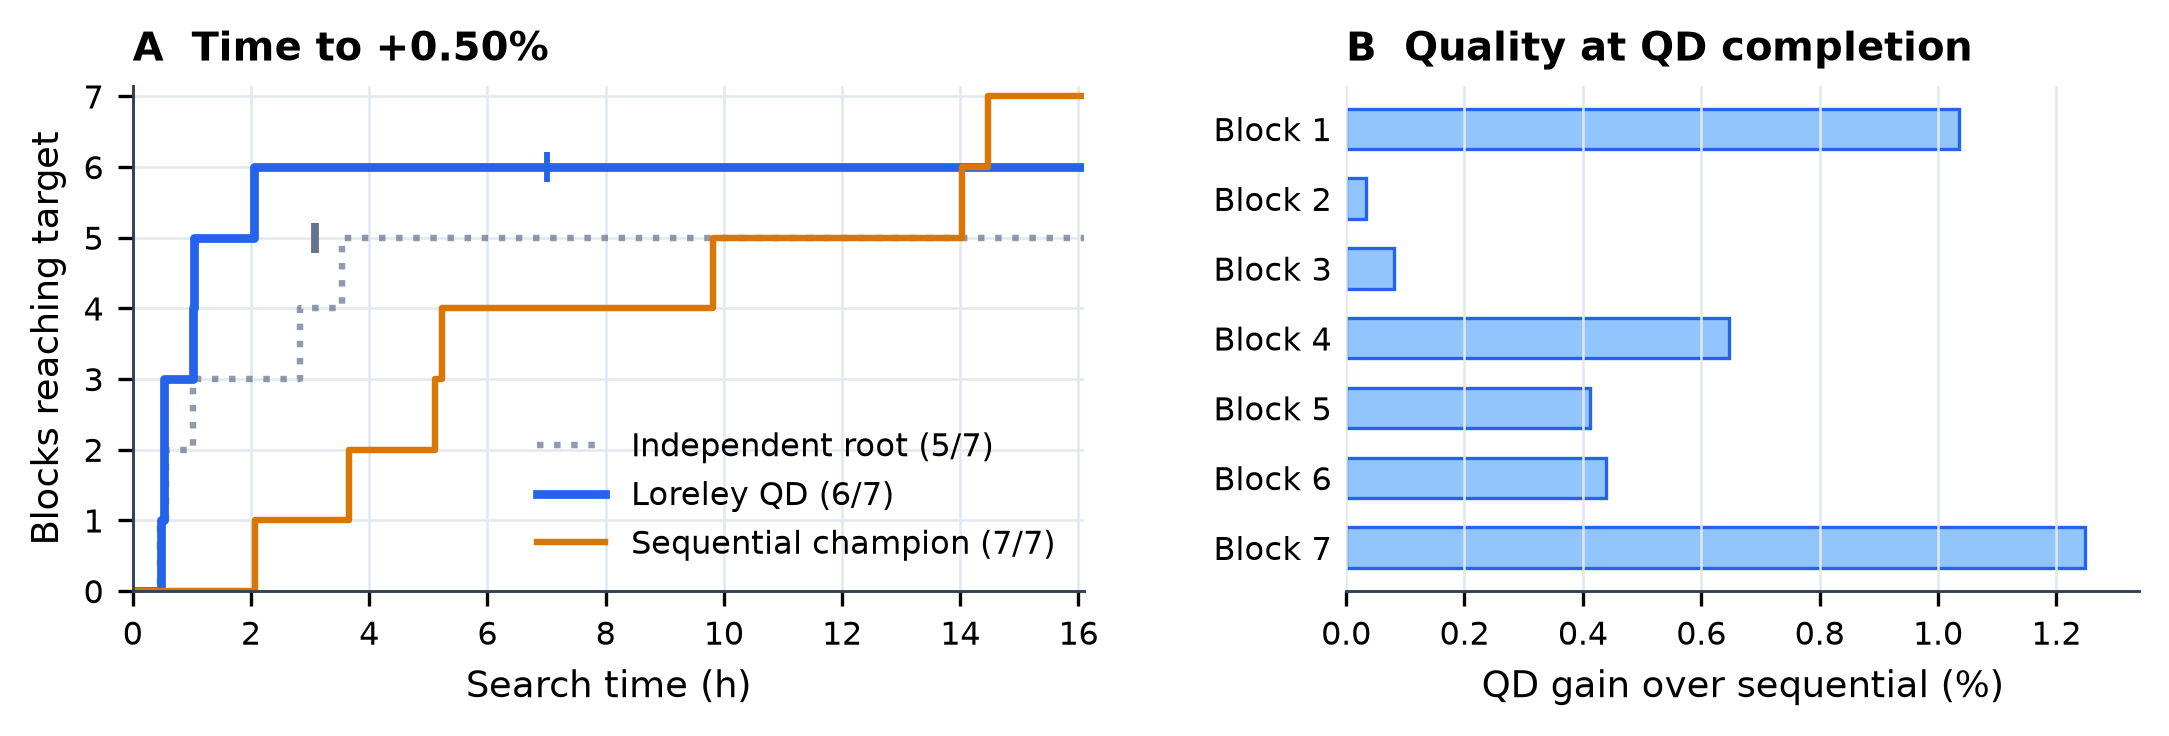
\includegraphics[width=0.985\textwidth]{figures/quality_time_en.png}
\end{center}
\vspace{2pt}

\begin{minipage}[t]{0.48\textwidth}
{\color{ink}\large\bfseries Time to $+0.50\%$}\par
\small
The experiment uses a $+0.50\%$ compression-throughput gain as the threshold for a useful improvement. First attainment is read from each block's recorded checkpoints:
\vspace{3pt}

\begin{tabularx}{\linewidth}{@{}Y r r@{}}
\toprule
Strategy & Blocks & Median time \\
\midrule
\textbf{Loreley QD} & \textbf{6/7} & \textbf{0.78 h} \\
Sequential Champion & 7/7 & 5.23 h \\
\bottomrule
\end{tabularx}

\vspace{3pt}
QD is faster in all 6 blocks where both strategies reach the threshold. The paired geometric mean of Champion / QD attainment time is $6.76\times$. Times range from 0.48--2.05 h for QD and 2.08--14.46 h for Sequential Champion.

\vspace{5pt}
{\color{ink}\bfseries The critical path explains the time gap}\par
QD runs 4 candidates concurrently, with median effective parallelism of 3.37. Sequential Champion runs one at a time, with median effective parallelism of 0.99. Total queue time per strategy and block is about 3--7 minutes, far below the hours separating them. QD advances several branches at once; Sequential Champion follows a single dependency chain.
\end{minipage}\hfill
\begin{minipage}[t]{0.48\textwidth}
{\color{ink}\large\bfseries Equal jobs and equal time}\par
\small
\colorbox{orangepale}{\parbox{\dimexpr\linewidth-2\fboxsep\relax}{%
\vspace{3pt}\textbf{At 48 jobs, Sequential Champion finishes higher.}\par
Mean holdout gains are $+0.96\%$ for Sequential Champion, $+0.82\%$ for QD, and $+0.50\%$ for Independent Root. Sequential Champion has the highest mean endpoint at this fixed job count.\vspace{3pt}}}

\vspace{5pt}
\colorbox{bluepale}{\parbox{\dimexpr\linewidth-2\fboxsep\relax}{%
\vspace{3pt}\textbf{When QD finishes, it leads in all 7 blocks.}\par
When QD completes 48 jobs, Sequential Champion's latest recorded checkpoint is job 8 in 4 blocks, job 16 in 2 blocks, and job 24 in 1 block. QD scores higher in all 7, with a median paired advantage of $+0.44\%$.\vspace{3pt}}}

\vspace{5pt}
\colorbox{greenpale}{\parbox{\dimexpr\linewidth-2\fboxsep\relax}{%
\vspace{3pt}\textbf{Under a time limit, QD delivers better candidates.}\par
QD takes about as long as Independent Root while accumulating edits across generations. When delivery time matters, quality over wall-clock time is more informative than the endpoint after job 48 alone.\vspace{3pt}}}
\end{minipage}

\vspace{7pt}
{\color{muted}\scriptsize
Wall-clock time is reconstructed from 1,008 candidate-job timestamps and covers candidate search only. At each checkpoint, validation selects a candidate before holdout compression throughput is measured. There is no interpolation between checkpoints. Vertical markers indicate that the threshold was not reached within 48 jobs.}

\clearpage

% -----------------------------------------------------------------------------
% Page 3
% -----------------------------------------------------------------------------
\pagetitle{02 / LONGER SEARCHES}{New candidates in the second half}

\begin{center}
  % Self-contained raster charts avoid platform-specific font dependencies.
  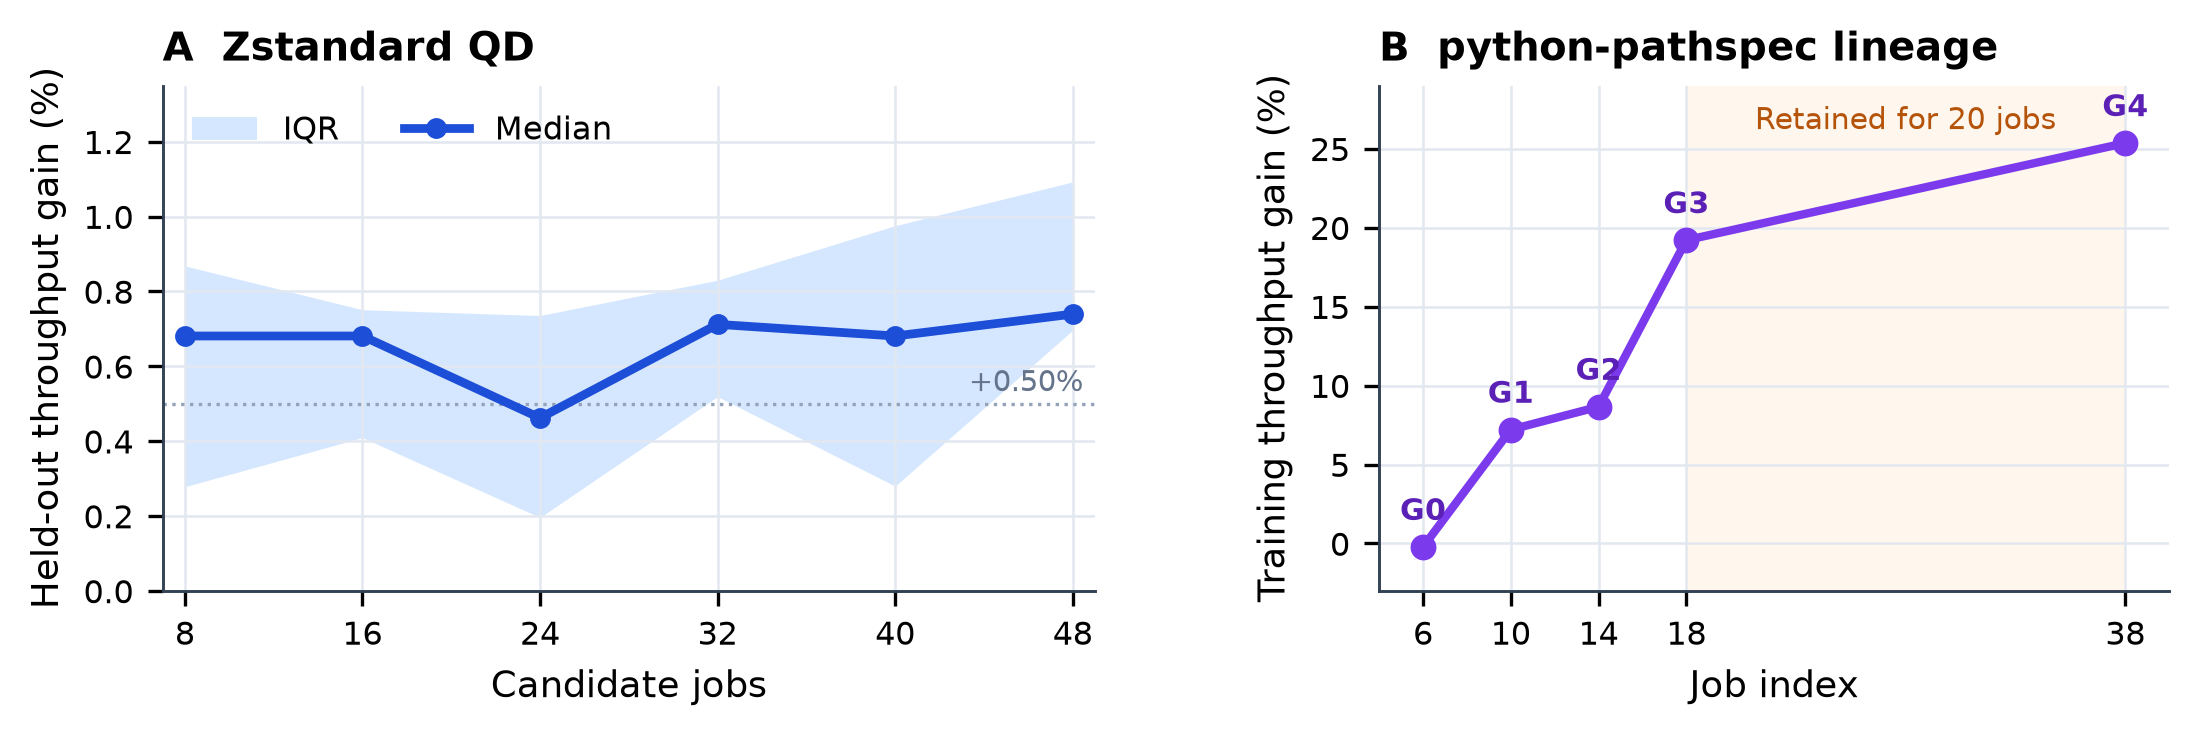
\includegraphics[width=0.985\textwidth]{figures/job_dynamics_en.png}
\end{center}
\vspace{3pt}

\colorbox{surface}{\parbox{\dimexpr\textwidth-2\fboxsep\relax}{%
\vspace{2pt}
\metriccard{20}{Distinct primary parents per block\par Median; range 15--23}{blue}\hfill
\metriccard{5.5}{Median job gap\par before a parent is selected again}{blue}\hfill
\metriccard{5--9}{Maximum generation\par reached across blocks}{green}\hfill
\metriccard{3--42}{Jobs between a retained branch\par and its final descendant}{orange}
\vspace{2pt}}}

\vspace{5pt}

\begin{minipage}[t]{0.48\textwidth}
{\color{ink}\large\bfseries Gains continue from jobs 24 to 48}\par
\small
Between jobs 24 and 48, the mean holdout gain of QD's selected candidates rises from $+0.47\%$ to $+0.82\%$, and the median from $+0.46\%$ to $+0.74\%$. Five of seven blocks improve; two remain unchanged. Three final candidates first appear at jobs 26, 38, and 43.\par
In the 220-job Zstandard run, every consecutive 16-job interval within the first 128 jobs adds a candidate to the archive. Jobs 129--220 add another 15 entries. The generation-4 candidate \texttt{fe39bee8} first appears at job 57 and achieves $+1.17\%$ on the existing holdout.
\end{minipage}\hfill
\begin{minipage}[t]{0.48\textwidth}
{\color{ink}\large\bfseries How the archive keeps search productive}\par
\small
In MAP-Elites, candidates compete within the same behavior cell. A state that is not the global leader can therefore remain available as a parent~\citep{mouret2015mapelites}. Loreley keeps a local Pareto front in each cell, preserving different trade-offs among compression, decompression, and worst-cell performance~\citep{pierrot2022mome}.\par
For two classes of combinatorial problems, Qian et al. prove that preserving intermediate states across cells lets MAP-Elites achieve polynomial expected runtime, while a globally competing evolutionary algorithm needs exponential expected time on some instances~\citep{qian2024qdhelpful}. Loreley's lineage records show non-leading branches being selected again after several jobs and producing better descendants.
\end{minipage}

\vspace{7pt}
\callout{Pathspec lineage}{A branch is retained after reaching $1.19\times$ at job 18. The next 20 jobs start from other branches. At job 38, the retained branch is selected again and produces a generation-4 candidate at $1.25\times$: a $+25.14\%$ gain on the reference workload.}

\clearpage

% -----------------------------------------------------------------------------
% Page 4
% -----------------------------------------------------------------------------
\pagetitle{03 / APPLICATION}{Wall-clock time and long-run gains}

{\color{ink}\large\bfseries Results on three complete repositories}\par
\small
\setlength{\tabcolsep}{5pt}
\renewcommand{\arraystretch}{1.18}
\begin{tabularx}{\textwidth}{@{}Y C{13mm} C{20mm} C{40mm} Y@{}}
\toprule
Target & Jobs & Final generation & Final candidate result & Search history \\
\midrule
\texttt{markdown-it-py} & 64 & 4 & Independent validation: $+6.75\%$ & Edits accumulate at jobs 7/12/14/26 \\
\texttt{python-pathspec} & 64 & 4 & Reference workload: $+25.14\%$ & Branch retained at job 18, continued at job 38 \\
Zstandard (long run) & 220 & 4 & Existing holdout: $+1.17\%$; fresh holdout: $+0.89\%$ & Candidate appears at job 57; 15 archive entries after job 128 \\
\bottomrule
\end{tabularx}

\vspace{7pt}
{\color{ink}\large\bfseries What this changes in engineering decisions}\par
\vspace{3pt}
\decisionbox{bluepale}{1. Report time to threshold}{When generation and evaluation can run in parallel, QD avoids putting all jobs on one champion chain. Here, QD reaches $+0.50\%$ sooner and leads Sequential Champion in all 7 blocks when its 48 jobs finish.}\hfill
\decisionbox{greenpale}{2. Track branch revisits}{To evaluate an archive, record how often parents are selected, the gaps between branch revisits, when final candidates first appear, and gains between checkpoints.}\hfill
\decisionbox{orangepale}{3. Compare both jobs and time}{At 48 jobs, Sequential Champion has the highest mean endpoint. At QD's completion time, QD leads in all 7 blocks. Report both comparisons.}

\vspace{7pt}
\begin{minipage}[t]{0.485\textwidth}
{\color{ink}\large\bfseries When this approach fits}\par
\small
\begin{itemize}
  \item Generating or evaluating one candidate takes minutes, and at least 3--4 candidates can run safely in parallel.
  \item Optimization requires compatible, cross-file edits over several generations.
  \item A project evaluator can check correctness, resource limits, and performance together.
  \item Complete Git states are needed for reproduction, rollback, and combining branches.
\end{itemize}
\end{minipage}\hfill
\begin{minipage}[t]{0.485\textwidth}
{\color{ink}\large\bfseries Summary}\par
\small
Loreley combines parallel candidate generation with a multi-branch archive that can be revisited. Parallel scheduling shortens the wall-clock time to a useful improvement. The archive keeps intermediate states that are not yet leaders, allowing later jobs to select them as parents and continue evolving them.\par
In these experiments, QD reaches the improvement threshold sooner and delivers better candidates within the same wall-clock time. Longer runs keep adding candidates in their later stages, and retained branches produce better descendants after gaps spanning many jobs. Loreley's strengths are faster access to useful results and continued gains during longer searches.
\end{minipage}

\vspace{6pt}
\colorbox{surface}{\parbox{\dimexpr\textwidth-2\fboxsep\relax}{%
\scriptsize\textbf{Data sources.}
Zstandard comparison records, reconstructed quality--time measurements, and long-run records from three repositories. Verification scripts cover 126 checkpoint selections, endpoint statistics, and lineage counts.}}

\vspace{3pt}
{\footnotesize
\setlength{\bibsep}{0pt}
\bibliographystyle{abbrvnat}
\bibliography{references}}

\end{document}
